\documentclass[11pt, oneside]{article}   	% use "amsart" instead of "article" for AMSLaTeX format


% \usepackage{draftwatermark}
% \SetWatermarkText{Draft}
% \SetWatermarkScale{5}
% \SetWatermarkLightness {0.9} 
% \SetWatermarkColor[rgb]{0.7,0,0}

\usepackage{geometry}                		% See geometry.pdf to learn the layout options. There are lots.
\geometry{letterpaper}                   		% ... or a4paper or a5paper or ... 
%\geometry{landscape}                		% Activate for for rotated page geometry
%\usepackage[parfill]{parskip}    		% Activate to begin paragraphs with an empty line rather than an indent
\usepackage{graphicx}				% Use pdf, png, jpg, or eps� with pdflatex; use eps in DVI mode
								% TeX will automatically convert eps --> pdf in pdflat						
								% TeX will automatically convert eps --> pdf in pdflatex		
\usepackage{amssymb}
\usepackage{mathrsfs}
\usepackage{hyperref}
\usepackage{url}
\usepackage{subcaption}
\usepackage{authblk}
\usepackage{amsmath}
\usepackage{mathtools}
\usepackage{graphicx}
\usepackage[export]{adjustbox}
\usepackage{fixltx2e}
\usepackage{hyperref}
\usepackage{alltt}
\usepackage{color}
\usepackage[utf8]{inputenc}
\usepackage[english]{babel}
\usepackage{float}
\usepackage{bigints}
\usepackage{braket}
\usepackage{siunitx}

%
% so you can do e.g., \begin{bmatrix}[r] (or [c] or [l])
%

\makeatletter
\renewcommand*\env@matrix[1][c]{\hskip -\arraycolsep
  \let\@ifnextchar\new@ifnextchar
  \array{*\c@MaxMatrixCols #1}}
\makeatother

\newcommand{\argmax}{\operatornamewithlimits{argmax}}
\newcommand{\argmin}{\operatornamewithlimits{argmin}}

\title{A Few Notes on Bell States, Superdense Coding, and Quantum Teleportation}
\author{David Meyer \\ dmm@\{1-4-5.net,uoregon.edu\}}

\date{Last update: \today}							% Activate to display a given date or no date



\begin{document}
\maketitle

\section{Introduction}

The Bell Circuit, shown in Figure \ref{fig:bell_circuit}, is comprised of two gates, $H$ and CNOT, which are defined as follows:

\begin{flalign*}
H = \frac{1}{\sqrt{2}}  \begin{bmatrix}[r] 1 & 1 \\ 1 &  -1 \end{bmatrix}, 
\text{CNOT} = \begin{bmatrix}[r] 
1 & 0 & 0 & 0 \\ 
0 & 1 & 0 & 0 \\
0 & 0 & 0 & 1 \\
0 & 0 & 1 & 0 \\
\end{bmatrix}
\end{flalign*}

\bigskip
\noindent
and results in two maximally entangled qubits\footnote{This state is sometimes called an \emph{EPR} state.}.
How does this work? 

\bigskip
\noindent
First, recall that

\begin{flalign*}
H \ket{0} &= \frac{1}{\sqrt{2}} \big ( \ket{0} + \ket{1} \big )  \text{ and }
H \ket{1} = \frac{1}{\sqrt{2}} \big ( \ket{0} - \ket{1} \big ) 
\end{flalign*}


\bigskip
\noindent
The Bell Circuit applies $H$ to $\ket{b_0}$ and then applies the CNOT gate to $H\ket{b_0}$ (control qubit)  
and $\ket{b_1}$ (target qubit). The inputs and evolution of the Bell Circuit are shown are Table \ref{tab:bell_state}.

\bigskip
\begin{figure}
\center{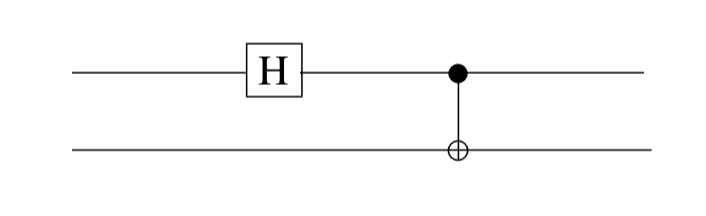
\includegraphics[scale=0.45, frame] {images/bell_forward_circuit.png}}
\caption{Bell Circuit}
\label{fig:bell_circuit}
\end{figure}

\begin{table}[H]
\centering
\begin{tabular}{c | c | c | c | c}
$b_{0} b_{1}$  & $H \ket{b_0}$ & $\ket{b_1}$ & Bell Circuit evolution with inputs $\ket{b_0}$ and $\ket{b_1}$  & Bell State\\
\hline
00  & $H\ket{0}$ & $\ket{0}$ & $\ket{0} \xrightarrow{\scriptsize H}  \frac{1}{\sqrt{2}} (\ket{0} + \ket{1}) 
  \xrightarrow{\otimes \ket{0}}  \frac{1}{\sqrt{2}} (\ket{0} + \ket{1}) \ket{0} \xrightarrow{\scriptsize \text{CNOT}} \frac{1}{\sqrt{2}} (\ket{00} + \ket{11})$ & $\ket{\phi^+}$ \\
01  & $H\ket{0}$ & $\ket{1}$ & $ \ket{0} \xrightarrow{\scriptsize H} \frac{1}{\sqrt{2}} (\ket{0} + \ket{1})  
  \xrightarrow{\scriptsize \otimes \ket{1}} \frac{1}{\sqrt{2}} (\ket{0} + \ket{1})  \ket{1} \xrightarrow{\scriptsize \text{CNOT}}  \frac{1}{\sqrt{2}} (\ket{01} + \ket{10})$\ & $\ket{\psi^+}$ \\
10  & $H\ket{1}$ & $\ket{0}$ & $\ket{1} \xrightarrow{\scriptsize H}  \frac{1}{\sqrt{2}} (\ket{0} - \ket{1})  \xrightarrow{\scriptsize \otimes \ket{0}} \frac{1}{\sqrt{2}} (\ket{0} - \ket{1})  \ket{0} \xrightarrow{\scriptsize \text{CNOT}} \frac{1}{\sqrt{2}}  (\ket{00} - \ket{11})$ & $\ket{\phi^-}$ \\
11    & $H\ket{1}$ & $\ket{1}$ & $\ket{1} \xrightarrow{\scriptsize H}  \frac{1}{\sqrt{2}} (\ket{0} - \ket{1}) 
  \xrightarrow{\scriptsize \otimes  \ket{1}}  \frac{1}{\sqrt{2}} (\ket{0} - \ket{1})  \ket{1} \xrightarrow{\scriptsize \text{CNOT}} \frac{1}{\sqrt{2}}  (\ket{01} - \ket{10})$ & $\ket{\psi^-}$
\end{tabular}
\caption{Bell States}
\label{tab:bell_state}
\end{table}

\bigskip
\noindent
What we can see from Table \ref{tab:bell_state} is that $b_0$ selects the "bit" ($\ket{\phi}$ or $\ket{\psi}$), and $b_1$ selects the "sign" ($\ket{+}$ or $\ket{-}$). Since there
are four orthonormal states, the \emph{Bell basis}, we can encode two bits ($b_0$ and $b_1$) in the four Bell States.  

\bigskip
\noindent
Now,  if Alice wants to send two classical bits to  Bob (\emph{superdense coding}) using one qubit, she need only transform her qubit\footnote{Her half of the EPR pair, the two entangled qubits.} 
into the Bell State corresponding to the two bits she wants to send, then send her half to Bob (this requires a \emph{quantum} channel). Bob can then recover Alice's two bit message.


\bigskip
\noindent
But how can Bob recover Alice's message? Recall that unitary quantum operations are reversible. So Bob can use the Reverse Bell Circuit shown in Figure \ref{fig:reverse_bell_circuit} to recover
Alice's 2 bit message.


\bigskip
\begin{figure}[H]
\center{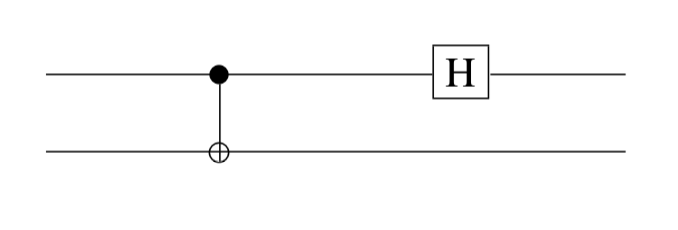
\includegraphics[scale=0.45, frame] {images/bell_reverse_circuit.png}}
\caption{Reverse Bell Circuit}
\label{fig:reverse_bell_circuit}
\end{figure}

\section{Superdense Coding}

Suppose Alice wants to send Bob the message $00$. Alice can perform one or more unitary operations on her qubit (her half of the entangled pair) that will allow Bob, 
when presented with Alice's qubit, to reconstruct Alice's message $b_0b_1$. If we run $\ket{\phi^+}$ through the circuit in Figure \ref{fig:reverse_bell_circuit},
that is, $\ket{\phi^+}  \xrightarrow {\scriptsize \text{CNOT}}  \xrightarrow {\scriptsize \text{  H  }}  \ket{b_0b_1}$,  Bob will recover Alice's message ($b_0b_1 = 00$). Why is this?

\begin{flalign*}
\ket{\phi^+} &=  \frac{1}{\sqrt{2}} (\ket{00} + \ket{11}) \longrightarrow  \\
& \frac{1}{\sqrt{2}} (\ket{0}  \ket{0} + \ket{1} \ket{1}) \xrightarrow {\scriptsize \text{CNOT}} \frac{1}{\sqrt{2}} (\ket{00} + \ket{10}) \longrightarrow \\
& \frac{1}{\sqrt{2}} (\ket{00} + \ket{10}) \xrightarrow {\scriptsize \text{  H  }}  \frac{1}{\sqrt{2}}  \Big ( \frac{1}{\sqrt{2}}  (\ket{0} + \ket{1}) \ket{0} + \frac{1}{\sqrt{2}}  (\ket{0} - \ket{1}) \ket{0} \Big) \\
&= \frac{1}{\sqrt{2}} \frac{1}{\sqrt{2}}  \Big ( (\ket{0} + \ket{1}) \ket{0} + (\ket{0} - \ket{1}) \ket{0} \Big ) \\
&= \frac{1}{2} \big (\ket{00} + \ket{10} + \ket{00} - \ket{10} \big ) \\
&= \frac{1}{2} \big  (2 \ket{00} + (\ket{10} - \ket{10}) \big ) \\
&=  \frac{1}{2} \cdot 2 \ket{00} \\
&= \ket{00}
\end{flalign*}


\bigskip
\noindent
Bob can now measure both qubits and recover Alice's message ($b_0b_1 = 00$). 


\bigskip
\noindent
In general, Alice notices that 

\begin{itemize}
\item To send \textbf{00}, apply the Identity matrix $\mathbf{I} = \begin{bmatrix} 1 & 0 \\ 0 & 1 \end{bmatrix}$ to her half of the EPR pair
\item To send \textbf{01}, apply the matrix $\mathbf{X} = \begin{bmatrix} 0 & 1 \\ 1 & 0 \end{bmatrix}$ to her half of the EPR pair
\item To send \textbf{10}, apply the matrix $\mathbf{Z} = \begin{bmatrix}[r] 1 & 0 \\ 0 & -1 \end{bmatrix}$ to her half of the EPR pair
\item To send \textbf{11}, apply $i\mathbf{Y} = i \begin{bmatrix}[r] 0 & -i \\ i & 0 \end{bmatrix}$, i.e. both $\mathbf{X}$ and $\mathbf{Z}$,  to her half of the EPR pair
\end{itemize} 

\bigskip
\noindent
where $\mathbf{I}$, $\mathbf{X}$, $\mathbf{Y}$ and $\mathbf{Z}$ are the \emph{Pauli} matrices \cite{wiki:pauli_matrices}. 
\bigskip
\noindent
This transforms the EPR pair $\ket{\phi^+}$ into the four Bell States $\ket{\phi^+}$, $\ket{\psi^+}$, $\ket{\phi^-}$ and $\ket{\psi^-}$ respectively:

\begin{itemize}
\item \textbf{00}: $\begin{bmatrix} 1 & 0 \\ 0 & 1 \end{bmatrix}  \frac{1}{\sqrt{2}} (\ket{00} + \ket{11} \longrightarrow  \frac{1}{\sqrt{2}} (\ket{00} + \ket{11}) =
\frac{1}{\sqrt{2}} \begin{bmatrix} 1 \\ 0 \\  0 \\ 1 \end{bmatrix} = \ket{\phi^+}$

\item \textbf{01:} $\begin{bmatrix} 0 & 1 \\ 1 & 0 \end{bmatrix} \frac{1}{\sqrt{2}} (\ket{00} + \ket{11} \longrightarrow  \frac{1}{\sqrt{2}} (\ket{01} + \ket{10}) =
\frac{1}{\sqrt{2}} \begin{bmatrix} 0 \\ 1 \\  1 \\ 0 \end{bmatrix} = \ket{\psi^+}$

\item \textbf{10:} $\begin{bmatrix}[r] 1 & 0 \\ 0 & -1 \end{bmatrix}  \frac{1}{\sqrt{2}} (\ket{00} - \ket{11} \longrightarrow  \frac{1}{\sqrt{2}} (\ket{00} - \ket{11}) =
\frac{1}{\sqrt{2}} \begin{bmatrix}[r] 1 \\ 0 \\  0 \\  -1 \end{bmatrix} = \ket{\phi^-}$

\item \textbf{11:}  $i  \begin{bmatrix}[r] 0 & -i \\ i & 0 \end{bmatrix} \frac{1}{\sqrt{2}} (\ket{00} + \ket{11} \longrightarrow  \frac{1}{\sqrt{2}} (\ket{01} - \ket{10}) =
\frac{1}{\sqrt{2}} \begin{bmatrix}[r] 0 \\ 1 \\  -1 \\ 0 \end{bmatrix} = \ket{\psi^-}$
\end{itemize}

\bigskip
\noindent
The four Bell states $\ket{\phi^+}$, $\ket{\psi^+}$, $\ket{\phi^-}$ and $\ket{\psi^-}$ are orthonormal and are hence distinguishable by 
quantum measurement.  Thus after receiving Alice's transformed qubit (her half of the EPR pair),
Bob can measure both qubits and recover $b_0b_1$. Hence one qubit carries two classical bits of information; this is superdense coding.
We saw an example of this above in which Bob recovered $\ket{00}$ from $\ket{\phi^+}$ using 
the Reverse Bell Circuit depicted in Figure \ref{fig:reverse_bell_circuit}.

\subsection{Aside: Spectral Decomposition of Pauli Matrices}
So far we've interpreted the Pauli matrices as a quantum gates. But note that a gate such \textbf{Z} is a Hermitean operator and as a 
result can be interpreted as an observable. Somewhat surprisingly (notice the symmetry),  the spectral decomposition \cite{2014arXiv1405.5749S}
 of \textbf{Z}  is

\begin{flalign*}
\mathbf{Z} =  \ket{0}\bra{0} - \ket{1}\bra{1}
\end{flalign*}

\bigskip
\noindent
where  $\ket{u}\bra{v}$ is Dirac notation \cite{2000RPPh...63.1893G} for the outer product $\mathbf{u} \otimes \mathbf{v} =  \mathbf{u} \mathbf{v}^{\text{T}}$ of $m \times 1$ vector 
\textbf{u} and  $n \times 1$ vector \textbf{v}, which yields a $m \times n$ matrix\footnote{The outer product is of vectors 
\textbf{u} and \textbf{v}  is a special case of the tensor product  $\mathbf{u} \otimes \mathbf{v}$. 
More generally, the outer product is an instance of a Kronecker product \cite{wiki:kronecker}.}.



\bigskip
\noindent
We can see that the eigenvalues of \textbf{Z}  are 1 and -1, corresponding to eigenvectors $\ket{0}$  and $\ket{1}$  respectively. So the measurement operators are the 
projectors $\ket{0}\bra{0}$ and $\ket{1}\bra{1}$,  This means that a measurement of the Pauli observable \textbf{Z} is a measurement in the computational basis that has 
eigenvalue +1 corresponding to $\ket{0}$  and eigenvalue -1 corresponding to $\ket{1}$. 

\bigskip
\noindent
So ok, but why does $\mathbf{Z} = \ket{0}\bra{0} - \ket{1}\bra{1}$? Well, we know that the outer product $\mathbf{u} \otimes \mathbf{v}$ of a $m \times 1$ vector  \textbf{u} and a 
$n \times 1$ vector  \textbf{v} is defined to be the $m \times n$ matrix\footnote{Contrast with the scalar inner product  
$\langle \mathbf{u},  \mathbf{v} \rangle = \mathbf{u}^{\text{T}} \mathbf{v}$. Note also that $\langle \mathbf{u},  \mathbf{v} \rangle = \text{tr}(\mathbf{u} \otimes \mathbf{v})$,
where $\text{tr}(\mathbf{A})$ is the "trace" of matrix \textbf{A}. } $\mathbf{u} \mathbf{v}^{\text{T}}$.

\bigskip
\noindent
To see why $\mathbf{Z} = \ket{0}\bra{0} - \ket{1}\bra{1}$, first recall that  $\ket{0} = \begin{bmatrix} 1 \\0 \end{bmatrix}$ and $\ket{1} = \begin{bmatrix} 0 \\ 1 \end{bmatrix}$. Then

\begin{flalign*}
\ket{0}\bra{0}  &= \begin{bmatrix} 1 \\ 0 \end{bmatrix} \begin{bmatrix} 1 \\ 0 \end{bmatrix}^{\text{T}} =
\begin{bmatrix} 1 \\ 0 \end{bmatrix} \begin{bmatrix} 1  & 0 \end{bmatrix} = \begin{bmatrix} 1 & 0 \\ 0 & 0 \end{bmatrix} \text{ and} \\
\ket{1}\bra{1}  &= \begin{bmatrix} 0 \\ 1 \end{bmatrix}\begin{bmatrix} 0 \\ 1 \end{bmatrix}^{\text{T}}  = \begin{bmatrix} 0 \\ 1 \end{bmatrix} \begin{bmatrix} 0  & 1 \end{bmatrix} = \begin{bmatrix} 0 & 0 \\ 0 & 1 \end{bmatrix} \text{ so that} \\
\ket{0}\bra{0} - \ket{1}\bra{1} &= \begin{bmatrix} 1 & 0 \\ 0 & 0 \end{bmatrix}  - \begin{bmatrix} 0 & 0 \\ 0 & 1 \end{bmatrix} = \begin{bmatrix}[r] 1 & 0 \\ 0 & -1 \end{bmatrix} = \mathbf{Z}
\end{flalign*}


\bigskip
\subsection{Back to Alice wanting to send a message to Bob}
Now suppose Alice want's to send Bob the message 01.  Alice then applies Pauli matrix $X$ to $\ket{\phi+}$ to get $\ket{\psi^+}$:

\begin{equation*}
\mathbf{X} \ket{\phi^+} = \begin{bmatrix}[r] 0 & 1  \\ 1 & 0\end{bmatrix} \frac{1}{\sqrt{2}} (\ket{00} + \ket{11} = \frac{1}{\sqrt{2}} (\ket{01} + \ket{10}) = \ket{\psi^+}
\end{equation*}

\bigskip
\noindent
Bob can now recover Alice's message as follows using the Reverse Bell Circuit (Figure \ref{fig:reverse_bell_circuit}). That is, Bob can
do the the unitary operations $\ket{\psi^+}  \xrightarrow {\scriptsize \text{CNOT}}  \xrightarrow {\scriptsize \text{H}}  \ket{01}$, as follows:


\begin{flalign*}
\ket{\psi^+} &= \frac{1}{\sqrt{2}} (\ket{01} + \ket{10}) \longrightarrow \\
& \frac{1}{\sqrt{2}} (\ket{0}  \ket{1} + \ket{1} \ket{0}) \xrightarrow {\scriptsize \text{CNOT}} \frac{1}{\sqrt{2}} (\ket{01} + \ket{11}) \longrightarrow \\
& \frac{1}{\sqrt{2}} (\ket{01} + \ket{11}) \xrightarrow {\scriptsize \text{  H  }}  \frac{1}{\sqrt{2}}  \Big ( \frac{1}{\sqrt{2}}  (\ket{0} + \ket{1}) \ket{1} + \frac{1}{\sqrt{2}}  (\ket{0} - \ket{1}) \ket{1} \Big) \\
&= \frac{1}{\sqrt{2}} \frac{1}{\sqrt{2}}  \Big ( (\ket{0} + \ket{1}) \ket{1} + (\ket{0} - \ket{1}) \ket{1} \Big ) \\
&= \frac{1}{2} \big (\ket{01} + \ket{11} + \ket{01} - \ket{11} \big) \\
&= \frac{1}{2} \big (2 \ket{01} + (\ket{11} - \ket{11}) \big) \\
&=  \frac{1}{2}  \cdot 2 \ket{01} \\
&=  \frac{2}{2}  \ket{01} \\
&= \ket{01}
\end{flalign*}

\bigskip
\noindent
Now Bob can measure the two qubits and recover Alice's message ($b_0b_1 = 01$).

\bigskip
\noindent
Similarly, suppose Alice wants to send the message 10 to Bob. Alice first transforms her qubit as follows


\begin{equation*}
\mathbf{Z} \ket{\phi^+} = \begin{bmatrix}[r] 1 & 0 \\ 0 & -1 \end{bmatrix}  \frac{1}{\sqrt{2}} (\ket{00} + \ket{11} = \frac{1}{\sqrt{2}} (\ket{00} -  \ket{11}) = \ket{\phi^-}
\end{equation*}

\bigskip
\noindent
Alice now sends her qubit to Bob over a quantum channel. Bob can now recover Alice's message, again using the Reverse Bell Circuit 
($\ket{\phi^-}  \xrightarrow {\scriptsize \text{CNOT}}  \xrightarrow {\scriptsize \text{  H  }}  \ket{10}$). Again, why is this?

\begin{flalign*}
\ket{\phi^-} &=  \frac{1}{\sqrt{2}} (\ket{00} - \ket{11}) \longrightarrow \\
& \frac{1}{\sqrt{2}} (\ket{0}  \ket{0} - \ket{1} \ket{1}) \xrightarrow {\scriptsize \text{CNOT}} \frac{1}{\sqrt{2}} (\ket{00} - \ket{10}) \longrightarrow \\
& \frac{1}{\sqrt{2}} (\ket{00} - \ket{10}) \xrightarrow {\scriptsize \text{  H  }}  \frac{1}{\sqrt{2}}  \Big ( \frac{1}{\sqrt{2}}  (\ket{0} + \ket{1}) \ket{0} -  \frac{1}{\sqrt{2}}  (\ket{0} - \ket{1}) \ket{0} \Big) \\
&= \frac{1}{\sqrt{2}} \frac{1}{\sqrt{2}}  \Big ( (\ket{0} + \ket{1}) \ket{0} -  (\ket{0} - \ket{1}) \ket{0} \Big ) \\
&= \frac{1}{2} \big (\ket{00} + \ket{10} - \ket{00}  + \ket{10} \big ) \\
&= \frac{1}{2} \big (2 \ket{10} + (\ket{00} - \ket{00}) \big ) \\
&=  \frac{1}{2} \cdot 2 \ket{10} \\
&= \ket{10}
\end{flalign*}

\bigskip
\noindent
Now Bob can measure the two qubits and recover Alice's message ($b_0b_1 = 10)$.

\bigskip
\noindent
Finally, if Alice wants to send $11$ to Bob she first transforms her qubit 

\begin{equation*}
i \mathbf{Y} \ket{\phi^+} =  \begin{bmatrix}[r] 0 & -i \\ i & 0 \end{bmatrix}   \frac{1}{\sqrt{2}} (\ket{00} + \ket{11} = \frac{1}{\sqrt{2}} (\ket{01} - \ket{10}) = \ket{\psi^-}
\end{equation*}

\bigskip
\noindent
Alice now transmits her qubit to Bob and Bob applies the Reverse Bell Circuit to recover Alice's message:

\begin{flalign*}
\ket{\psi^-} &= \frac{1}{\sqrt{2}} (\ket{01} -  \ket{10}) \longrightarrow \\
& \frac{1}{\sqrt{2}} (\ket{0}  \ket{1} - \ket{1} \ket{0}) \xrightarrow {\scriptsize \text{CNOT}} \frac{1}{\sqrt{2}} (\ket{01} -  \ket{11}) \longrightarrow \\
& \frac{1}{\sqrt{2}} (\ket{01} -  \ket{11}) \xrightarrow {\scriptsize \text{  H  }}  \frac{1}{\sqrt{2}}  \Big ( \frac{1}{\sqrt{2}}  (\ket{0} + \ket{1}) \ket{1} - \frac{1}{\sqrt{2}}  (\ket{0} - \ket{1}) \ket{1} \Big) \\
&= \frac{1}{\sqrt{2}} \frac{1}{\sqrt{2}}  \Big ( (\ket{0} + \ket{1}) \ket{1} -  (\ket{0} - \ket{1}) \ket{1} \Big ) \\
&= \frac{1}{2} \big (\ket{01} + \ket{11} -  \ket{01} +  \ket{11} \big) \\
&= \frac{1}{2} \big (2 \ket{11} + (\ket{01} - \ket{01}) \big) \\
&=  \frac{1}{2}  \cdot 2 \ket{11} \\
&=  \frac{2}{2}  \ket{11} \\
&= \ket{11}
\end{flalign*}

\bigskip
\noindent
Now Bob can measure the two qubits and recover Alice's message ($b_0b_1 = 11)$.


\section{Quantum Teleportation}
Quantum teleportation can be thought of as the dual task to super dense coding. Whereas super dense coding is concerned with conveying classical information 
via a qubit, quantum teleportation is concerned with conveying quantum information with classical bits \cite{Bennett:1992tv}.

\subsection{A high-level view of the quantum teleportation algorithm}

\begin{enumerate}
\item Alice and Bob share an entangled (EPR) pair $\ket{\phi^+}$
\item Alice chooses a qubit $\ket{\psi}$ as the message she wants to convey to Bob
\item Alice performs operations on $\ket{\psi}$ and $\ket{\phi^{+}_A}$ (Alice's her half of $\ket{\phi^+}$)
\item Alice measures $\ket{\psi}$  and her half of  $\ket{\phi^+_A}$, destroying both of her qubits
\item Alice sends the two classical bits that were the results of her measurements to Bob
\item Bob uses the two classical bits to "correct" $\ket{\phi^{+}_B}$ (his half of $\ket{\phi^+}$) to be $\ket{\psi}$
\end{enumerate}

\bigskip
\noindent
Alice uses the circuit in Figure \ref{fig:a_reverse_bell_circuit} to prepare her two qubits (step 3 above). How exactly does this work? 
First, notice that the input to the Reverse Bell Circuit shown in Figure \ref{fig:a_reverse_bell_circuit} is $\ket{\psi} \otimes \ket{\phi^{+}_A}$. 
To see how this works, first recall that $\ket{\psi} = \alpha \ket{0} + \beta \ket{1}$.  Then 


\begin{figure}[t]]
\center{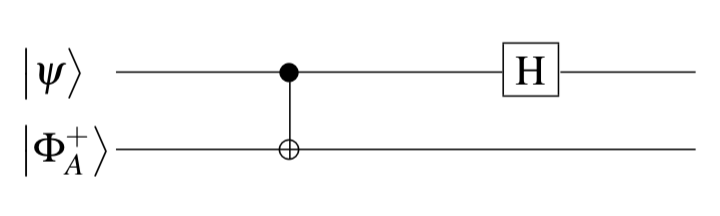
\includegraphics[scale=0.45, frame] {images/a_reverse_bell_circuit.png}}
\caption{Reverse Bell Circuit}
\label{fig:a_reverse_bell_circuit}
\end{figure}

\begin{flalign*}
\ket{\psi} \otimes \ket{\phi^{+}_A} &= (\alpha \ket{0} + \beta \ket{1}) \otimes \frac{1}{\sqrt{2}} (\ket{00} + \ket{11}) \\
&= \frac{1}{\sqrt{2}} \Big ( \alpha (\ket{000} + \alpha \ket{011}) + \beta (\ket{100} + \ket{111}) \Big ) \xrightarrow {\scriptsize \text{CNOT}}  
\quad\qquad \mathrel{\#} \ket{b_0b_1b_2}: b_0 \text{ is control, } b_1  \text{ is target} \\
& \frac{1}{\sqrt{2}} \Big ( \alpha \ket{000} + \alpha \ket{011})+ \beta (\ket{110} + \ket{101}) \Big ) \xrightarrow {\scriptsize \text{H}}  
\; \qquad \qquad\qquad \mathrel{\#} \text{apply $H$ to $b_0$} \\
& \frac{1}{\sqrt{2}} \bigg [ \alpha \Big ( \frac{1}{\sqrt{2}} \ket{0} + \ket{1} \Big ) \ket{00} + \alpha \Big (  \frac{1}{\sqrt{2}} \ket{0} + \ket{1}) \Big )  \ket{11}  + 
\beta \Big ( \frac{1}{\sqrt{2}} \ket{0} - \ket{1} \Big ) \ket{10} + \beta \Big (  \frac{1}{\sqrt{2}} \ket{0} - \ket{1} \Big )  \ket{01}  \bigg ]\\
&= \frac{1}{\sqrt{2}} \frac{1}{\sqrt{2}}  
\bigg [ \alpha \Big ( \big (\ket{0} + \ket{1} \big ) \ket{00} +  \big (\ket{0} + \ket{1} \big )  \ket{11} \Big)  +
\beta \Big ( \big (\ket{0} - \ket{1} \big ) \ket{10} + \big ( \ket{0} - \ket{1} \big )  \ket{01} \Big ) \bigg] \\
&= \frac{1}{2} \bigg [ \alpha \Big (\ket{000} + \ket{100}  +  \ket{011} + \ket{111}) \Big)  +
\beta \Big (\ket{010} - \ket{110} + \ket{001} - \ket{101}  \Big ) \bigg ] \\
&= \frac{1}{2} \bigg [ \alpha \ket{000} + \alpha \ket{100}  +  \alpha \ket{011} + \alpha \ket{111})  +
 \beta \ket{010} - \beta\ket{110} + \beta \ket{001} - \beta \ket{101}  \bigg ] \\
\end{flalign*}

\bigskip
\noindent
Now Alice measures her two qubits ($\ket{\psi} \otimes \ket{\phi^{+}_A} $) and observes $b_0b_1 \in \{00, 01, 10, 11\}$ with $P(b_0b_1) = \frac{1}{4}$. 


\bigskip
\noindent
Now here's the amazing thing. If Alice observes $00$, she communicates this to Bob (over a classical channel). As soon as
Bob sees the value $00$, he knows that his qubit $\ket{\phi^{+}_{B}} = \alpha \ket{0} + \beta \ket{1}$. How does Bob know this?

\bigskip
\noindent
First, as shown above

\begin{flalign}
\label{eqn:psi_otimes_phi+}
\ket{\psi} \otimes \ket{\phi^+} = \frac{1}{2} \bigg [ \alpha \ket{000} + \alpha \ket{100}  +  \alpha \ket{011} + \alpha \ket{111})  +
\beta \ket{010} - \beta\ket{110} + \beta \ket{001} - \beta \ket{101}  \bigg ] 
\end{flalign}
 
 
 \bigskip
\noindent
Alice's measurement of the first two qubits collapses Bob's qubit to the third qubit\footnote{Recall that the original three qubits were
$\ket{\psi} \otimes \ket{\phi^{+}_{AB}}$.}.  The only terms in Equation \ref{eqn:psi_otimes_phi+} that are 
consistent with the first two qubits being $\ket{00}$ (resulting from Alice's measurement)
are $\alpha \ket{000}$ and $\beta \ket{001}$. The "collapsed version" is $\alpha \ket{0}$ and $\beta \ket{1}$. 
Hence Bob knows that his qubit, $\ket{\phi^{+}_B}$,  equals $\alpha \ket{0} + \beta \ket{1}$.

 \bigskip
\noindent
Since Alice sent the two bits she saw to Bob, he knows which operations to perform to transform $\ket{\phi^{+}_B} \rightarrow \ket{\psi}$.  
In particular, $b_0 = 1$ Bob should apply Pauli matrix $Z$ to his qubit and $I$ otherwise, 
and if $b_1 = 1$ he should apply $X$ and $I$ otherwise. This transforms $\ket{\phi^{+}_B}$, Bob's qubit, into $\ket{\psi}$. 
This is shown in Table \ref{tab:bob}.

\bigskip
\noindent
Amazingly  this procedure teleports Alice's qubit $\ket{\psi}$ to Bob using the two classical bits that Alice learned by measuring her two qubits ($\ket{\psi}$ and $\ket{\phi^{+}_A}$).  

\bigskip
\begin{table}[H]
\centering
\begin{tabular}{c | c | r | r}
$b_{0} b_{1}$  & $\ket{\phi^{+}_B}$  & \multicolumn{1}{c|}{Transformation} & \multicolumn{1}{c}{Computation}  \\
\hline
\textbf{00}  & $\alpha \ket{0} + \beta \ket{1}$ & $\mathbf{I} \begin{bmatrix} \alpha \\ \beta \end{bmatrix}$ & $\begin{bmatrix} 1 & 0 \\ 0 & 1 \end{bmatrix} 
 \begin{bmatrix} \alpha \\ \beta \end{bmatrix}  = \begin{bmatrix} \alpha \\  \beta  \end{bmatrix} = \alpha \ket{0} + \beta \ket{1} = \ket{\psi}$  \\
\textbf{01}  & $\beta \ket{0} + \alpha \ket{1}$ & $\mathbf{X}\begin{bmatrix} \beta \\ \alpha  \end{bmatrix}$ & $ \begin{bmatrix} 0 & 1 \\ 1 & 0 \end{bmatrix}  \begin{bmatrix} \beta \\ \alpha  \end{bmatrix} 
= \begin{bmatrix} \alpha \\  \beta  \end{bmatrix}  = \alpha \ket{0} + \beta \ket{1} = \ket{\psi}$ \\
\textbf{10}  & $\alpha \ket{0} - \beta \ket{1}$ & $\mathbf{Z} \begin{bmatrix}[r]   \alpha \\  -\beta  \end{bmatrix}$ & $\begin{bmatrix}[r] 1 & 0  \\ 0 & -1 \end{bmatrix}  \begin{bmatrix}[r] \alpha \\ -\beta \end{bmatrix} 
= \begin{bmatrix} \alpha \\  \beta  \end{bmatrix}  = \alpha \ket{0} + \beta \ket{1} = \ket{\psi}$ \\
\textbf{11}  & $\beta \ket{0} - \alpha \ket{1} $ & $\mathbf{XZ} \begin{bmatrix}[r]  \beta \\  - \alpha  \end{bmatrix}$ & $  \begin{bmatrix} 0 & 1 \\ 1 & 0 \end{bmatrix}  \begin{bmatrix}[r] 1 & 0  \\ 0 & -1 \end{bmatrix} 
  \begin{bmatrix}[r] \beta \\ -  \alpha  \end{bmatrix} = \begin{bmatrix} \alpha \\  \beta  \end{bmatrix} = \alpha \ket{0} + \beta \ket{1} = \ket{\psi}$ \\
\end{tabular}
\caption{Bob's transformations on receiving classical bits $\mathbf{b_0b_1}$ from Alice}
\label{tab:bob}
\end{table}


\subsection{Curious Entry for \textbf{11} in Table \ref{tab:bob}?}
Note that the row for the result of Alice's measurement \textbf{11} in Table \ref{tab:bob} is curious. When Bob sees \textbf{11} from Alice he knows that his remaining qubit 
$\ket{\psi^{+}_B}$, equals $- \beta \ket{0} + \alpha \ket{1}$. Why does the table say $\beta \ket{0} - \alpha \ket{1}$? 

\bigskip
\noindent
Here is one way to look at this: First,
recall that when Bob receives classical bits \textbf{11} from Alice he knows that his qubit, $\ket{\psi^{+}_B}$,  is

\begin{flalign*}
\ket{\psi^{+}_B} &= - \beta \ket{0} + \alpha \ket{1} = \begin{bmatrix} -\beta \\ \alpha \end{bmatrix}
\end{flalign*}

\bigskip
\noindent
Now, if Bob now wants to transform $\ket{\psi^{+}_B} \rightarrow \ket{\psi}$, he would apply $\mathbf{ZX}$ as follows

\begin{flalign*}
\mathbf{ZX} \ket{\psi^{+}_B}  &=  \begin{bmatrix}[r] 1 & 0  \\ 0 & -1 \end{bmatrix}   \begin{bmatrix} 0 & 1 \\ 1 & 0 \end{bmatrix}  \begin{bmatrix} -\beta \\ \alpha \end{bmatrix} \\
&= \begin{bmatrix}[r] 1 & 0  \\ 0 & -1 \end{bmatrix}   \begin{bmatrix} \alpha \\ - \beta \end{bmatrix} \\
&= \begin{bmatrix} \alpha \\ \beta \end{bmatrix} \\
&= \alpha \ket{0} + \beta \ket{1} \\
&= \ket{\psi}
\end{flalign*}


\bigskip
\noindent
But our rule (Table \ref{tab:bob})  tells Bob to apply $\mathbf{XZ}$ when he sees \textbf{11} from Alice. Why? Notice the following:


\begin{flalign*}
\mathbf{ZX} \begin{bmatrix} x_0 \\ x_1 \end{bmatrix} &= \mathbf{Z} \begin{bmatrix} x_1 \\ x_0  \end{bmatrix} =  \begin{bmatrix}[r] x_1 \\  - x_0 \end{bmatrix} \\
\mathbf{XZ} \begin{bmatrix} x_0 \\ x_1 \end{bmatrix} &= \mathbf{X} \begin{bmatrix}[r] x_0 \\ - x_1  \end{bmatrix}  = \begin{bmatrix}[r] - x_1 \\  x_0 \end{bmatrix}  
\end{flalign*}


\bigskip
\noindent
which implies that

\bigskip

\begin{equation}
\mathbf{ZX} \begin{bmatrix} x_0 \\ x_1 \end{bmatrix}  = - \mathbf{XZ} \begin{bmatrix} x_0 \\ x_1 \end{bmatrix}
\label{eqn:equal}
\end{equation}

\bigskip
\bigskip
\noindent
So now let $x_0 = \beta$ and $x_1 =   \alpha$.  Then

\begin{flalign*}
\mathbf{XZ} \Big [\beta \ket{0} - \alpha \ket{1} \Big ] = \mathbf{XZ} \begin{bmatrix}[r] \beta  \\ - \alpha \end{bmatrix} = \mathbf{X} \begin{bmatrix} \beta \\ \alpha \end{bmatrix} 
=  \begin{bmatrix} \alpha \\ \beta \end{bmatrix} = \alpha \ket{0} + \beta \ket{1} = \ket{\psi}
\end{flalign*}

\bigskip
\noindent
and $- \big (\beta \ket{0} - \alpha \ket{1} \big )= -\beta \ket{0} + \alpha \ket{1} \longrightarrow$

\begin{flalign*}
\mathbf{ZX}  \Big [ -\beta \ket{0} + \alpha \ket{1} \Big ] = \mathbf{ZX} \begin{bmatrix}[r] - \beta \\ \alpha \end{bmatrix} = \mathbf{Z} \begin{bmatrix}[r] \alpha \\ - \beta\end{bmatrix} 
 = \begin{bmatrix} \alpha \\ \beta \end{bmatrix} = \alpha \ket{0} + \beta \ket{1} = \ket{\psi}
 \end{flalign*}

\bigskip
\bigskip
\noindent
The choice of the transformation rules shown in Table \ref{tab:bob} and Equation \ref{eqn:equal} allows us to write 
$\beta \ket{0} - \alpha \ket{1}$ rather than $- \beta \ket{0} + \alpha \ket{1}$.

\bigskip
\noindent
Why do this? One thing it does is make the symmetry in Table \ref{tab:bob} more explicit, but hopefully there is a better reason...


\subsubsection{Cloning and/or Faster Than Light Communication?}
First, no faster-than-light communication occurs since Bob learns nothing from the changes until Alice actually sends the two classical bits to him (even
though Alice operating on $\ket{\phi^{+}_A}$ instantly affects $\ket{\phi^{+}_B}$).

\bigskip
\noindent
The No-Cloning Theorem \cite{2018arXiv180804213E}  is not violated since, even though Bob has an exact copy of $\ket{\psi}$, Alice had to destroy her copy (by
measuring it). 

\bigskip
\noindent
Finally, an interesting point is that neither Alice or Bob ever "know"  what $\ket{\psi}$ is (in terms of its actual amplitudes); all they know
is that it was transferred (whatever it was). 

\section{Bell and  CHSH}

\bigskip
\noindent

\section{Acknowledgements}

\newpage
\bibliographystyle{plain}
\bibliography{/Users/dmm/papers/bib/qc}



\end{document} 
